%%%%%%%%%%%%%%%%%%%%%%%%%%%%%%%%%%%%%%%%%%%%%%%%%%%%%%%%%%%%%%%%%%%%%%
%%%%  POOKA %%%%%%%%%%%%%%%%%%%%%%%%%%%%%%%%%%%%%%%%%%%%%%%%%%%%%%%
%%%%%%%%%%%%%%%%%%%%%%%%%%%%%%%%%%%%%%%%%%%%%%%%%%%%%%%%%%%%%%%%%%%%%%

\mysubsection{Pooka Virtues}{advancement-pooka-virtues}

\begin{center}
\myredbold{Unless otherwise specified, you can only take each Virtue once.}
\end{center}


  \mytable{Y Y Y} {
    \thead{Daredevil (Level 2+)} & \thead{Heroic (Level 4+)} & \thead{Legendary (Level 7+)} \\
  } {
    Apprentice of the Rabbit & Epic Songs & Kismet III \\
    Calling in the Markers & Fast Metabolism &  Martyrdom \\
    Fortunate &  Footpad of the Rabbit &  Personality III \\
    Healing Wax & Kismet II  &  Saga of Heroes \\
    Kismet I & Personality II & Saves III \\
    Laugh it Off & Rager & Sharper of the Rabbit \\
    Must Be My Lucky Day! & Saves II & -  \\
    Personality I & Wound Transfer & - \\
    Saves I  & - & - \\
    Two Murks Walk Into a Bar... & - & - \\
}


\begin{multicols*}{2}


\myhighlight{Apprentice of the Rabbit}{adv-pooka-apprentice-rabbit}

Gain the rank of Apprentice (d4) in the \mylink{Whispers of Br'er Rabbit}{vulgate-whisper-brer-rabbit}.

\myhighlight{Calling in the Markers}{adv-pooka-markers}

During the \mylink{Shopping Step}{downtime-shopping} of \mylink{Downtime}{downtime}, you can roll your \LUCK. You gain up to \SUM items from the \mylink{Tools}{gear-equipment} list, as long as the total cost doesn't exceed \SUM x10 gold.  If you wish, you can distribute this gear immediately to the rest of your Band.

\myhighlight{Epic Songs}{adv-pooka-epic-songs}

When using your \mylink{Hype Man}{pooka-virtue-hype-man} Virtue, you roll a d8 for each member of your Band (including yourself).

\myhighlight{Fast Metabolism}{adv-pooka-fast-metabolism}

You are immune to \mylink{Toxins}{malignants-toxins}, \mylink{Curses}{cunning-curses}, and \mylink{Diseases}{vulgate-medicine-diseases} of all sorts.

\begin{center}
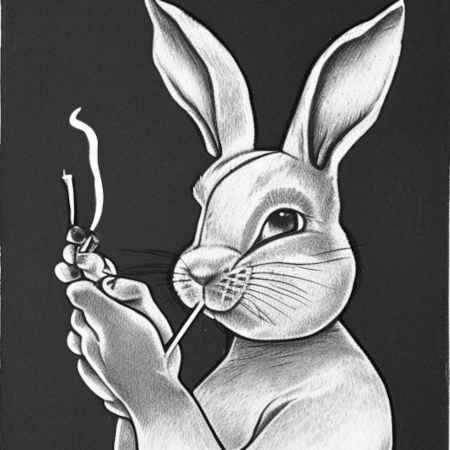
\includegraphics[scale=.4]{advancement/Pooka2}
\end{center}

\newpage

\myhighlight{Footpad of the Rabbit}{adv-pooka-footpad-rabbit}

Gain the rank of Footpad (d6) in the \mylink{Whispers of Br'er Rabbit}{vulgate-whisper-brer-rabbit} (you do not need to know Apprentice of the Rabbit).

\myhighlight{Fortunate}{adv-pooka-fortunate}

Advance your \mylink{Lucky Die}{pooka-lucky-die} \DCUP.

\myhighlight{Healing Wax}{adv-pooka-healing}

Once per Session, you can pull a glob of wax out of your ear.  Anyone who eats it restores 4 Flesh (up to \MAX). If no one consumes it by the end of the Session, it just becomes a "normal" lump of ear wax.

\myhighlight{Kismet I-III}{adv-pooka-kismet}

Advance \mybold{all} aspects of your \mylink{Kismet}{adventurer-kismet} to the next named level (\DEATH, \INJURY, or \INSANITY).

\myhighlight{Laugh it Off}{adv-pooka-laugh-it-off}

Once per Session, you may make it so that any physical blow that would hit you misses instead.  This has to be plausible and luck based: "I slipped and fell just as the sword came down and it missed me", for instance.  You can choose to "laugh it off" after the damage is rolled.

\myhighlight{Martyrdom}{adv-pooka-martyrdom}

If a Mortal Ally dies, you can take their place.  The Ally needs to be Close or Nearby to you, and they cannot have been dead for longer than Hours.  The body of the Mortal must be in reasonably good shape - you can't save them if they've been reduced to ashes, for example.  You immediately disappear into the Void and the Ally's soul returns immediately to its body. Those who have been saved by Pooka are said to take on some of their "personality".

\cbreak

\myhighlight{Must Be My Lucky Day!}{adv-pooka-lucky-day}

 Once per \mylink{Session}{time-session}, you can do 1 of the following:  (a) win any game of chance; (b) find extra Narcotics just lying around (d2 \UD of any Narcotic you want - if you don't use it before the next Session, it gets lost or evaporates or whatever); (c) find a \mylink{Tool}{gear-equipment} you might need lying on the ground. The tool can only be used once before it breaks, is used up, etc.; or (d) regain 1 Flesh (enough to bring you off Death's Door).

\myimage{advancement/LittleWitch}


\myhighlight{Personality I-III}{advancement-pooka-personality}

Advance two \mybold{different} aspects of your \mylink{Personality}{adventurer-personality} \DCUP.

\myhighlight{Rager}{adv-pooka-rager}

Once per Session, you can host a Rager during a \mylink{Bivouac}{combat-resting}.  Every person who participates will gain the effects of the \mylink{Resting Step}{downtime-resting} of \mylink{Downtime}{downtime}. The following morning, everyone must make an \RSTRY{\VIG}. If they fail they are \mylink{Hung Over}{effect-hung-over}.

\newpage

\myhighlight{Saga of Heroes}{adv-pooka-saga-heroes}

When using your \mylink{Hype Man}{pooka-virtue-hype-man} Virtue, you roll a d10 for each member of your Band (including yourself).

\myhighlight{Saves I-III}{adv-pooka-saves}

Advance \mybold{all} \mylink{Saves}{adventurer-saves} to the next named level (Defenseless to Preserved; Preserved to Protected; etc).

\myhighlight{Sharper of the Rabbit}{adv-pooka-sharper-rabbit}

Gain the rank of Sharper (d8) in the \mylink{Whispers of Br'er Rabbit}{vulgate-whisper-brer-rabbit} (you do not need to know Apprentice or Footpad of the Rabbit).


\cbreak

\myhighlight{Two Murks Walk Into a Bar...}{adv-pooka-two-murks}

When using your \mylink{Hype Man}{pooka-virtue-hype-man} Virtue, you roll a d6 for each member of your Band (including yourself).

\myhighlight{Wound Transfer}{adv-pooka-wound-transfer}

You can transfer your Flesh to Allies on a 1-to-1 basis i.e. for every point of Flesh you transfer, you take 1 point of Flesh damage. You do not need to be touching the Ally, but you do need to be Close to them.  The wounds that appear on your body match the wounds taken by the Ally.  The point of Flesh transferred is enough to keep an Ally from Dying.

\end{multicols*}
